\documentclass[article,type=msc,colorback,accentcolor=tud9c,twoside,11pt]{tudthesis}
\usepackage{titlesec}

%\usepackage{german}
\usepackage{amsmath}
\usepackage{algorithm}
\usepackage{tocloft}
\usepackage{chngcntr}
\counterwithin{figure}{section}
\usepackage[normalem]{ulem}
\usepackage{wrapfig}
\usepackage{amsmath}
\usepackage{algpseudocode}
%\usepackage[ansinew]{inputenc}
\newcommand{\getmydate}{%
  \ifcase\month%
    \or Januar\or Februar\or M\"arz%
    \or April\or Mai\or Juni\or Juli%
    \or August\or September\or Oktober%
    \or November\or Dezember%
  \fi\ \number\year%
}    
\usepackage{hyperref}
\usepackage{multirow}
\usepackage{float}
\usepackage{caption}
\usepackage[ngerman,english]{babel}
\usepackage{listings}
\usepackage{color}

\definecolor{dkgreen}{rgb}{0,0.6,0}
\definecolor{gray}{rgb}{0.5,0.5,0.5}
\definecolor{mauve}{rgb}{0.58,0,0.82}

\lstset{frame=tb,
  language=Java,
  aboveskip=3mm,
  belowskip=3mm,
  showstringspaces=false,
  columns=flexible,
  basicstyle={\small\ttfamily},
  numbers=none,
  numberstyle=\tiny\color{gray},
  keywordstyle=\color{blue},
  commentstyle=\color{dkgreen},
  stringstyle=\color{mauve},
  breaklines=true,
  breakatwhitespace=true,
  tabsize=3
}
\usepackage{tikz}
\usetikzlibrary{shapes.geometric, arrows}
\tikzstyle{startstop} = [rectangle, rounded corners, minimum width=1.5cm, minimum height=0.5cm,text centered, draw=black, fill=red!30]
\tikzstyle{io} = [trapezium, trapezium left angle=70, trapezium right angle=110, minimum width=1.5cm, minimum height=0.5cm, text centered, draw=black, fill=blue!30]
\tikzstyle{process} = [rectangle, minimum width=1.5cm, minimum height=0.5cm, text centered, draw=black, fill=orange!30]
\tikzstyle{decision} = [diamond, minimum width=3cm, minimum height=0.5cm, text centered, draw=black, fill=green!30]
\tikzstyle{arrow} = [thick,->,>=stealth]
\tikzstyle{connector} = [circle, rounded corners, minimum width=1.5cm, minimum height=0.5cm,text centered, draw=black, fill=yellow!30]


\begin{document}
\pagenumbering{roman}
  \thesistitle{OpenDiabetesVault: Data Gathering and Data Slicing Algorithms}
    {Master Thesis}
  \author{Ankush Chikhale}
 % \birthplace{Darmstadt}
  \referee {Prof. Dr. Max M{\"u}hlh{\"a}user}{Jens Heuschkel}
  \department{Fachbereich Informatik}
  \group{Telecooperation Group}
  \dateofexam{31 August, 2017}{31 August, 2017}
  %\tuprints{12345}{1234}
  \makethesistitle
  \affidavit{Ankush Chikhale}
  %\setlength{\parindent}{2em}
\setlength{\parskip}{1em}
\setcounter{secnumdepth}{5}
%\renewcommand{\baselinestretch}{1.0}
 
%\large
\index{key}

\cleardoublepage
\selectlanguage{ngerman} 
\begin{abstract}
 
\end{abstract}
\selectlanguage{english} 
\begin{abstract}
There is a need to download bulk amount of data from CareLink\textsuperscript{\textregistered} website. Carelink, Web-based system is designed to help take information from all of diabetes management tools such as insulin pump, continuous glucose monitor, blood glucose meter(s), and logbook - and organize it into easy-to-read charts, graphs and tables. This data will be used to generate pattern with the help of machine learning algorithm. The requirement is to make data available for researchers easily without actually visiting the website and this process is done with the help of Crawling methodology.
Crawling is the process through which we collect varieties of web pages, in order to gather information from them. It is the system for bulk downloading of web pages. It is a program or automated script, which browses the web in  automated manner. Using Web Crawler we are building a Native Java application for downloading and uploading bulk amount of data to and from server.
There is also need to upload data from local USB to server of website. This process is being handled by automating web browser control. we have utilized capability of Java with Selenium for automation Browser that helps in uploading data to server.
The thesis also tries to solve the problem of data slicer by building an algorithm, which recognize series of events depending on some criteria and saves the sliced data into local DB. For data  slicing, algorithm is built in Java and uses JDBC and sql with pub sub complex event system for recognition of events. For complex event system in Java JMS (Java messaging service) is used. JMS is a Java Message Oriented Middleware (MOM) API for sending messages between two or more clients. It is an implementation to handle the Producer-consumer problem. GUI based Native Java application is built with Framework of Swing. At the same time Command line project is being built with the help of Apache Commons CLI. Additionally JSoup as a Java framework is used to crawl website and visit particular page with ability to manipulate entries. In our application, Jsoup act as a Data crawler. All the tedious Programming automation is done to make upload and download task user friendly, simple and one click. Once the data is downloaded and uploaded, data validation and verification is done with the help of researcher working on Data mining Technologies. 
\end{abstract}

\clearpage
\tableofcontents 
\clearpage
\listoffigures
\clearpage
\listoftables
\listofalgorithms

\clearpage
\pagenumbering{arabic}
\selectlanguage{English}
\section{Introduction}
Data mining is the process for extraction of hidden predictive information from large databases. It is a powerful new technology with great potential to help companies focus on the most important information in their data warehouses. Researchers in TK Lab have a task of generating pattern or prediction from large amount of Medical data using Machine Learning and data mining. To capitalize the task of Data mining in field of Medical sector, we need bulk amount of data. This data will be provided from CareLink\textsuperscript{\textregistered} website. 

Carelink, Web-based system is designed to help take information from all of diabetes management tools such as insulin pump, continuous glucose monitor, blood glucose meter(s), and logbook - and organize it into easy-to-read charts, graphs and tables. These reports can help health care provider discover trends and other information that can lead to improved therapy management for greater control\footnote{https://carelink.minimed.eu/}.
Data crawler is required to access the required data from website without manually visiting it. Crawling is the process through which we collect varieties of web pages, in order to gather information from them. Especially with respect to Search Engines, crawlers are used to add index to web pages and it helps in building a database of web sites. It is the system for bulk downloading of web pages. It is a program or automated script, which browses the web in automated manner. Main prominent use of Web crawlers\footnote{http://webcourse.cs.technion.ac.il/236620/Winter2006-2007/ho/WCFiles/lec14-crawlers.PDF} are
\begin{enumerate}
\item	Data crawling, where web pages are analyzed for statistical properties.
\item	Web Search Engines.
\item	Web Archiving, where web pages are collected for successors.
\end{enumerate}
There are various types of crawlers available:
\begin{enumerate}
\item	Incremental crawlers: These type of crawlers continuously crawl their crawl space, to get fresh content.
\item	Batch crawlers: Crawl a snapshot of their crawl space, till a certain web site is reached.
\item	Focused crawlers: crawl pages to only restricted topics.
\end{enumerate}
Given the overwhelming use of crawler in different scenarios, Web Data crawling as a prominent use case for crawling is used in our research project to extract data for Medical research. URL for Carelink Website which has been crawled for extracting information is \textit{https://carelink.minimed.eu/}

Parallel to extracting data from website, we also have a need to upload data from local system or USB device to server. The process of uploading data to server is done in website using Applet. Since we cannot take Applet\cite{Javaapplet} out from browser and run it as stand alone due to signing and loin cookies issue, we try to automate the process of accessing applet in Web browser. Selenium\footnote{http://www.seleniumhq.org/} helps to automate browsers and simulate user interaction. It enables java program to emulate user interaction with a web page. Selenium\cite{Webdriver} uses Web Drivers for interacting with a Web browser. Web drivers helps to control web browsers by a hook and which in turn enables selenium to interact with web browsers similar to User. There are a numerous commercial and open source tools available for assisting with the development of automation. Selenium is possibly the most widely used open source solution. With the help of selenium, we are trying to automate uploading Data from USB to server and cut the human repeatable work. This will help mass upload of data with minimum efforts and time.

We have used Web bases technologies and Web data crawling added with automation technologies to make the entire process of data uploading and downloading smooth and easy with just one click. JSoup\cite{Jsoup} as a Java framework is used to crawl website and visit particular page with ability to manipulate entries. Jsoup is a java HTML parser. It is a java library that is used to parse HTML\cite{BeaqleJSHTML} document. Jsoup provides API to extract and manipulate data from URL or HTML file. It uses DOM, CSS and JQuery-like methods for extracting and manipulating file. This is used to download CSV file with user-entered dates. Jsoup will help in checking login credentials of User and will help in bypassing browser agent so that crawling is uninterrupted. After successful login Using Jsoup user input dates will be inserted so that required CSV file will be downloaded. 

To Build GUI based Native Java application, Swing Framework is used. In particular we have used Scene Builder which is a JavaFx\cite{JavaFx} project. Scene Builder\footnote{http://www.oracle.com/technetwork/java/javase/downloads/javafxscenebuilder-info-2157684.html} is a visual layout tool which helps user build application user interfaces without coding. The good thing about scene builder is, user can simply drag and drop UI components, modify it's properties, apply styles to it and all this will produce FXML code for the layout created. FXML file created from the UI drag and drop can then be used in combination with Java project by binding UI to application logic. Addition to building GUI based application, we have a need to build a Command line interface for the project. To help making command line run different parts of entire project, Apache Commons CLI is being used. The Apache Commons CLI\footnote{https://commons.apache.org/proper/commons-cli/} library provides an API for parsing command line options passed to programs. It's also able to print help messages detailing the options available for a command line tool

\textbf{Data slicing add few lines here for data slicing}

\clearpage
\section{Background}
In this section, we provide an overview of Web crawler, Data crawler, Automation and Data slicing. We start by discussing Web crawler and Data crawler with respect to world wide web and extracting data from web pages. We then move ahead with automating Web browser and simulating user behavior using Selenium as a automation tool. At last, we explain the newly built algorithm for Data slicing and recognizing events for it.

\subsection{Basics of Web Crawling}

Web crawler\cite{WebCrawlerAReview} also known as Web spider or Web Robot is a program, which helps to browse the Web in an automated manner. The entire process is called web crawling or spidering. Web Crawlers helps in automating maintenance task on a Web site, such as validating HTML Codes. A related use case is web archiving where in large set of web pages are collected in a periodic time frame. The most important reason for web crawler is, World Wide Web is not a centrally managed repository of information rather it is combination of millions of independent web content providers. In other words web is combined together by set of agreed - upon protocol and data formats such as Hypertext Transfer Protocol (HTTP) , the Hypertext Markup Language (HTML) , the Domain Name Service (DNS) , the Transmission Control Protocol (TCP) and the robots exclusion protocol. 

Data miners or search engines have few of the available choices as : Adopting to a pull model which will proactively search the web for new information or try to establish a set of protocols making content providers to push content of interest to the aggregators. To become a Content provider is very easy as web servers are highly independent and hence the web protocols were initially extremely simple lowered the barrier even further, this simplicity is expressed by many as the reason why the web succeeded where earlier hypertext systems had failed. Push protocol might have made it more difficult to set of web protocols and hence raised the barrier of entry for content providers, while the pull model does not require any extra protocols. Similarly the pull model lowers the barrier of entry for content aggregators as well: Executing a crawler does not require any a prior buy-in from content providers.The push model requires a trust relationship between content provider and content aggregator, something that is not given on the web at large - The relationship between Introduction content providers and search engines is characterized by both mutual dependence and adversarial dynamics.

Figure \ref{fig:CrawlerAlgorithFlowchart}\footnote{http://www.cis.uni-muenchen.de/}, shows flowchart of Breadth search algorithm which is used in our work for Extracting relevant links and data:
\begin{figure}[h]
	\centering
	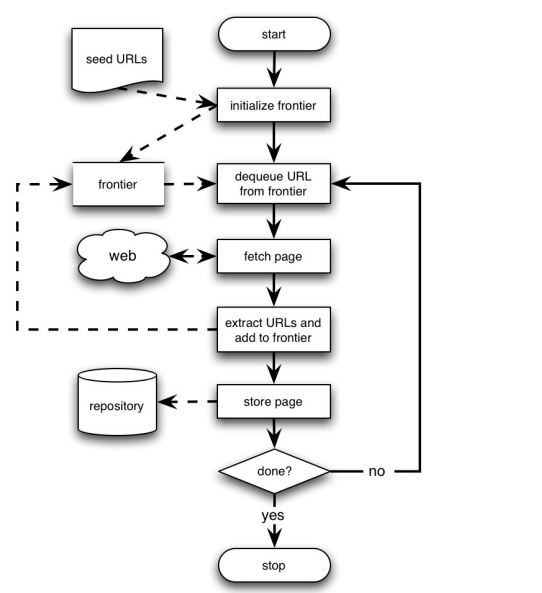
\includegraphics[scale=0.9]{CrawlerAlgorithFlowchart}
	\caption{Crawler Breadth search Flowchart}
	\label{fig:CrawlerAlgorithFlowchart}
\end{figure}
Even though the Web crawler algorithm is simple it still has few challenges\footnote{http://infolab.stanford.edu/} such as
\begin{enumerate}
\item Many content provider may try to add false information into the body generated by the crawler.
\item Most of the high throughput crawlers cannot crawl the entire web and they should not as crawling is performed carefully in controlled manner. There has to be balance between extraction of important content and exploitation of content already known to be useful.
\item Crawlers should follow "politeness" i.e not impose too much of a burden on the web sites they crawl.
\item Crawlers should achieve high throughput even though many website possess difficult structure for bot.
\end{enumerate}

Sometimes there might be case that crawlers visit web sites without approval or they consume resources on system. When crawling websites often issue of "politeness" comes into picture where large amount of pages are accessed. There are also new ways where in websites does not wished to be crawled to make this known to the crawling agent. There are large number of web pages on Internet and it makes the entire process highly complex. However, introduction of various modern Crawlers helps to solve this problem in a more sophisticated way.

\subsection{Crawler Architecture}

Web crawler consist of numerous process running on different machines interconnected by network. Multiple worker threads are created using crawler and loop work cycles are achieved using worker thread. Beginning of every work cycle, URL is fetched from Frontier Data structure,  which distributes URL according to policies mentioned such as politeness. Worker thread invokes the HTTP fetcher. To resolve host component of the URL into the IP address of relevant web server a DNS module is called using fetcher. It tries to connect to the web server, which checks for any robots exclusion rules and attempts to download the web page.
	
 When the download is completed, the web page can be stored in a repository of collected web page. Link extractor gets the page, which then parse the page HTML content and extracts hyperlinks contained within. Related URLs are passed to URL distributor, which assigns each URL to a crawling process. Most of the hyperlinks refer to pages on same website, assignment to local crawling process is common case. Now the URL is passed through URL filter and into the duplicate URL eliminator, which in turn maintains set of all URLs.  At last URL priotizer selects a position for the URL in the frontier, based on factors such as estimated page importance or rate of change.
 
Web Crawler needs to keep track of URL which are already visited and which needs to be visited. There is a flag associated with each URL whether page is downloaded or not. Few key functions should be taken into consideration such as Retrieving a URL, marking a URL as downloaded, adding a new URL and testing whether the set contains a URL. Modern web Crawler are splits into two main data structures as. 
 \begin{enumerate}
\item To maintain the set of URL that have been visited (duplicated URL eliminator)
\item To maintain set of URL that has to be visited (frontier)
\end{enumerate}

\subsubsection{Frontier Data Structure}
 Frontier \cite{frontierdatastructures} Data structure implements First in First out (FIFO).  Search technique used here is Breadth-first traversal of web graph. Most of the hyperlinks are relative and hence FIFO queue has long runs of URLs on same web server. Is it uncommon to not issue multiple overlapping request to server. The easiest way to realize it, is to maintain a mapping between web servers and crawling threads. A separate FIFO queue is assigned to each crawling thread. Another dedicated policy is, to send request to each web server depending on server's capabilities. For instance crawler can delay requests to a server by a multiple of time to get the last page from server. Mercator web crawler implements adaptive politeness. Frontier is divided into two parts, "front end" and "back end".

Front end consist of a single queue Q and URLs are added to the frontier by enqueuing them into that queue. Separate queues are contained in back end. Queue containing URL belongs to a single web server; mapping from back-end queues to web servers are maintained on table T. In addition, associated with each back-end queue q was a time t at which the next URL from q may be processed. These (q,t) pairs were organized into an in-memory priority queue, with the pair with lowest t having the highest priority.  Removing highest-priority entry (q,t) obtained URL by crawling thread from priority queue, waiting if necessary until time t had been reached, dequeuing the next URL u from q, downloading it, and finally reinserting the pair (q,tnow + k · x) into the priority queue, where now is the current time, x is the amount of time it took to download u, and k is a "politeness paramete"; typically 10. If dequeuing u from q left q empty, the crawling thread would remove the mapping from host(u) to q from T, repeatedly dequeue a URL u from Q and enqueue u into the back-end queue identified by T(host(u )), until it found a u such that host(u ) was not contained in T. At this point, it would enqueue u in q and update T to map host(u ) to q.
\subsubsection{URL Seen Test (duplicated URL eliminator)}
URL Seen Test is used to remove adding various instances of the similar URL to the frontier and therefore it is called duplicate URL eliminator. UST (URL Seen Test) supports insertion and set membership testing during batch crawling setting. There are various implementation of UST such as Bloom filter or hash table. In memory implementation has issues with scaling to large web corpora but they scale well in frontier. Commercial search engines employ distributed crawlers and a hash table realizing the UST can be partitioned across the machines in the crawling cluster.

Adding a bunch of URL into disk-based hash file involves reading the old hash file and writing out an updated version. Hence, the required time is directly equivalent to the number of discovered URLs. A slight improvement of this pattern is to store the URL hashes on disk in sorted order as before, but lightly packed rather than densely packed. The k highest-order bits of a hash determine the disk block where this hash resides. Merging a batch into the disk file is done in place, by reading a block for which there are hashes in the batch, checking which hashes are not present in that block, and writing the updated block back to disk. Thus, the time requirement for merging a batch is proportional to the size of the batch, not the number of discovered URLs. Once any block in the file fills up completely, the disk file is rewritten to be twice as large, and each block contains hashes that now share their k + 1 highest-order bits.

\subsubsection{Auxiliary Data Structures}
Web crawlers should follow Robots Exclusion protocol, a protocol that makes a web site admins to bar crawlers from crawling. It is done by providing a file at URL /robots.txt containing rules such as which pages the crawler is allowed to download. Before crawling web site crawler must check if the web site supplies /robots.txt file and if it does, crawler should adhere to rules. Some URLs contain a host component (e.g., www.yahoo.com), which is "resolved" using the Domain Name Service (DNS). DNS requests can take quite a long time due to the request forwarding nature of the protocol. Therefore, crawlers often maintain their own DNS caches. As with the robots exclusion rule cache, entries are expired according to both a standard eviction policy, and to expiration directives.
 
\subsubsection{Distributed crawling}

To increase the throughput of crawling, web crawler can be distributed over multiple machines. Distributed crawling is achieved by partitioning the URL space i.e. node is responsible for a subset of the URLs on the web. URL space is best partitioned across web site boundaries. Politeness policies are best achieved using partitioning the URL across site boundaries. In addition, most of the major data structures can be easily partitioned across site boundaries, i.e. the frontier, the DUE, the DNS and robots exclusion caches of each node contain URL, robots exclusion rules, and name-to-address mappings associated with the sites assigned to that node, and nothing else.

\subsubsection{Incremental crawling}
Snapshots of batch crawling can be combined using Web crawlers. To perform incremental or continuous crawling where the resources of the crawler are divided between downloading newly discovered pages. For making good Incremental crawling, requires few changes to the major data structures of crawlers. DUE should support deletion of URLs that are no longer valid. If URL are prioritized in frontier, the priority of a previously downloaded URL should be dependent on a model of the page's temporal behavior based on past observations. Other factors such as page quality are also taken into account.

\subsection{Selenium}
There are numerous browser automation tools available but the one, which outperforms others and could be found open source is Selenium. Selenium\cite{AutomationTestingAnIntroductiontoSelenium} is a browser automation tool; mostly it is used to simulate user interaction on web applications. The browser control is automated so that repetitive tasks can be automated. Selenium,  is a combination of selenium IDE, selenium Web driver and selenium gird. Selenium grid helps to use the selenium APIs to control browser instances distributed over a grid of machines. Selenium IDE is an extension for Firefox used to record and playback tests. Selenium uses lot of Jargon.

\begin{enumerate}
\item Selenium core JavaScript that control the browser.
\item Selenium WebDriver binds both language binding and individual browser controlling core.
\item Selenium RC is used for language binding.
\end{enumerate}

Advantages of Selenium:
\begin{enumerate}
\item Opensource tool
\item No licensing cost
\item Customize according to our requirement
\end{enumerate}

Disadvantage of selenium:
\begin{enumerate}
\item	There can be cases when selenium fails to recognize objects
\item Online support for selenium is very less
\end{enumerate}

Variant of selenium:
\begin{enumerate}
\item Selenium IDE
\item Selenium Core
\item Selenium Remote Control
\item Selenium Grid
\end{enumerate}

\subsubsection{WebDriver Design}
WebDrivers API \cite{SeleniumTestingFramework} is also called as  object-based. The interfaces are clearly defined and try to manage single responsibility and hence rather than modelling every single possible HTML Tag, we have only one WebElement interface. Snippet of code for initilization of web driver.\footnote{http://www.aosabook.org/en/selenium.html}

\begin{lstlisting}
WebDriver driver = new FirefoxDriver();
driver.<user hits space>
driver.findElement(<user hits space>);
driver.findElement(By.id("someid"));
\end{lstlisting}


\subsubsection{The IE Driver}
IE browser is constructed of a number of COM interfaces working in concert. JavaScript window is an IHTMLWindow.document is an instance of the COM interface  IHTMLDocument. Good thing about IE is that if COM classes works with IE6 it will still continue to work with IE9.

One of the main positives of IE design is that it does not need to have installer. So if there are no installer, there are consequences to this choice. IDE drivers built for selenium are tightly integrated with C\#. Even though c\# would be an attractive language to do the bulk of the coding in, it is not an good option. Something native for the communication to IE and therefor C++ as we don't need to use primary Interloop Assemblies (PIAs). Since we would need to run an installer in order to make that DLL available, we would link our library for communication with IE. In the figure  \ref{fig:OriginalIEdriver}, design of IEDriver is shown 
\begin{figure}[h]
	\centering
	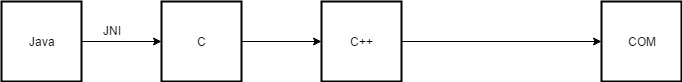
\includegraphics[scale=0.6]{OriginalIEdriver}
	\caption{Original IE driver}
	\label{fig:OriginalIEdriver}
\end{figure}

Looking at the diagram IE COM automation interfaces are being used and hence to make it easier to manage raw interfaces are wrapped with set of C++ classes that closely mirrored WebDriver API. For Java classes to communicate with C++ JNI is being used. This approach works well with java being only client language but could be very difficult if every other language would require to change the underlying library. Hence this is not the correct way for abstraction. Every other language had a mechanism of calling down straight C code. In c\# it is PInvoke, In ruby it is FFI, python has ctypes and Java it is JNA (Java Native Architecture). API has to be exposed to lowest common denominator and it was done by taking object model and flattening it, using a simple two or three letter prefix to indicate the "home interface" of the method: "wd" for "WebDriver" and "wde" for WebDriver Element. In Figure 
\ref{fig:ModifiedIEdriver}, design is shown 
\begin{figure}[h]
	\centering
	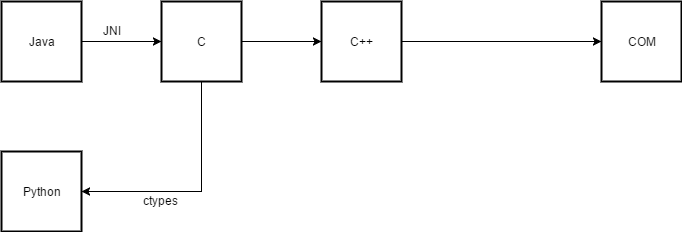
\includegraphics[scale=0.6]{ModifiedIEdriver.PNG}
	\caption{Modified IE driver}
	\label{fig:ModifiedIEdriver}
\end{figure}
On the Java side, we exposed this library of functions via an interface, which we then adapted to make it look like the normal object-oriented interface presented by WebDriver. For example, the Java definition of the getAttribute method looks like:

\begin{lstlisting}
public String getAttribute(String name) {
	PointerByReference wrapper = new PointerByReference();
	int result = lib.wdeGetAttribute(
			parent.getDriverPointer(), element, new WString(name), wrapper);
	errors.verifyErrorCode(result, "get attribute of");
	return wrapper.getValue() == null ? null : new StringWrapper(lib, wrapper).toString();
}
\end{lstlisting}

More and More of IE driver is being moved to sit upon the same automation Firefox. To achieve this we compile each of the atoms as c++ header file, exposing each function as constant. At last, we only have Interaction of API's in native code and rely on the atoms as much as possible.

\subsubsection{The Remote Driver}

To reduce the cost of maintaining web Driver by providing a uniform interface that language binding can code against is done with the help of Remote driver mechanism.To communicate with browser instance that is running out of process Remote driver is used. RPC mechanism is divided into two: transport and encoding. First iteration of the design was developed as a part of Firefox driver.

Mozilla, and therefore Firefox, was always seen as being a multi-platform application by its developers. Inspired by Microsoft's COM, Mozilla created a framework that allowed components to be built and bolted together called XPCOM (cross-platform COM).  IDL declares XPCOM interface, language binding for C and other languages and JavaScript as well as other languages are available. It's possible to make use of XPCOM objects in Firefox extensions because of the XPCOM consisting of JavaScript.

There are hardly any libraries available for custom protocol, hence they have to be built from the ground up for every language that we wanted to support. When we used to send only text line oriented protocol it was fine but when sending images started it was tedious.

Original RPC mechanism wasn't practical. Alternative for this was widely spread: HTTP. The Firefox driver is implemented as a Firefox extension, the basic design of which is shown in Figure above . HTTP server has been embedded into it. Writing HTTP servers in XPCOM wasn't one of our core areas to work on, so when the opportunity arose we replaced it with a basic HTTPD written by Mozilla themselves. Requests are received by the HTTPD and almost straight away passed to a dispatcher object.

\begin{figure}[h]
	\centering
	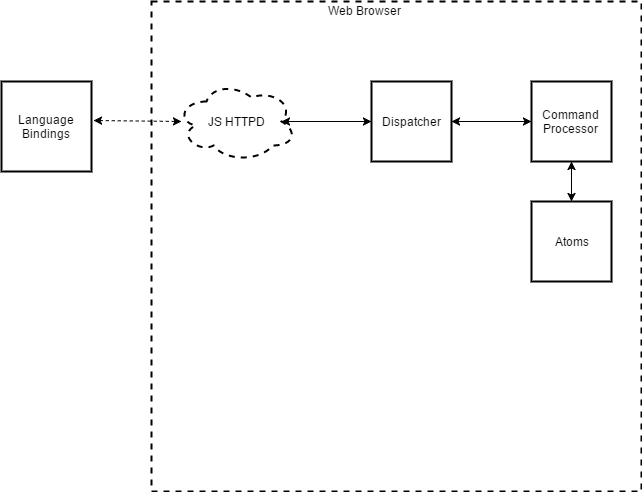
\includegraphics[scale=0.6]{SeleniumHttp.PNG}
	\caption{Firefox Driver Architecture}
	\label{fig:Flowchart}
\end{figure}

\begin{lstlisting}
{
  'name': 'getElementAttribute',
  'sessionId': { 'value': 'XXX' },
  'parameters': {
    'id': 'some_opaque_key',
    'name': 'rows'
  }
}
\end{lstlisting} 

This is then passed as a JSON string to a custom XPCOM component written called the CommandProcessor. Here's the code:
\begin{lstlisting}
var jsonResponseString = JSON.stringify(json);
var callback = function(jsonResponseString) {
  var jsonResponse = JSON.parse(jsonResponseString);

  if (jsonResponse.status != ErrorCode.SUCCESS) {
    response.setStatus(Response.INTERNAL_ERROR);
  }

  response.setContentType('application/json');
  response.setBody(jsonResponseString);
  response.commit();
};

// Dispatch the command.
Components.classes['@googlecode.com/webdriver/command-processor;1'].
    getService(Components.interfaces.nsICommandProcessor).
    execute(jsonString, callback);

\end{lstlisting}
Object above in code is converted into JSON string. A callback to the execute method that causes the HTTP response to be sent is passed.

 The "name" is been looked by execute method of the command processor which determines which function to call. The first parameter given to this implementing function is a "respond" object, which encapsulates not only the possible values that might be sent, but also has a method that allows the response to be dispatched back to the user and mechanisms to find out information about the DOM. The second parameter is the value of the parameters object seen above (in this case, id and name). The advantage of this scheme is that each function has a uniform interface that mirrors the structure used on the client side. This means that the mental models used for thinking about the code on each side are similar. Here's the underlying implementation of getAttribute,
 
 \begin{lstlisting}
FirefoxDriver.prototype.getElementAttribute = function(respond, parameters) {
  var element = Utils.getElementAt(parameters.id,
                                  respond.session.getDocument());
  var attributeName = parameters.name;

  respond.value = webdriver.element.getAttribute(element, attributeName);
  respond.send();
};
\end{lstlisting}

The first line simply looks up the element referred to by the opaque ID in a cache, In order to make element references consistent. In the Firefox driver, opaque ID is a UUID and the "cache" is simply a map. The getElementAt method checks whether referred to element is both known and attached to the DOM. If either check fails, the ID is removed from the cache (if necessary) and an exception is thrown and returned to the user.
The second line from the end makes use of the browser automation atoms discussed earlier, this time compiled as a monolithic script and loaded as part of the extension.
In last line, the send method is called. Simple check is done that only send a respone once before it calls the callback given to execute method. The response is sent back to the user in the form of a JSON string, which is decanted into an object that looks:
\begin{lstlisting}
{
  'value': '7',
  'status': 0,
  'sessionId': 'XXX'
}
\end{lstlisting}
Browsing the web in a copy of Firefox with the WebDriver extension installed will result in a bad security feature as it makes it trivially easy for someone to remotely control the browser.
There is a DOM messenger, waiting for the webdriver Command that reads the serialized JSON object and calls the execute method on the command processor. The callback is one that simply sets the response attribute on the document element and then fires the expected webdriverResponse event.

\subsubsection{Combinatorial Explosion}
There is challenge to minimize cost of maintenance with X browsers supporting Y languages, it would be trap of maintaining X*Y implementations. There can be a way to reduce the number of language that web driver support. It's always better to write automation scripts in the same language that they work on. There is also a way of reducing the supported browser but it will also not be a feasible solution
\subsubsection{Different Browsers}
Web browser is a translation device, which takes document written in HTML language and translates it into a formatted web page. The basic rules for translating HTML documents are established by the WWW. HTML standards usually run ahead of that the browsers support. Over the past few years Internet Explorer has done a lot than Opera or other browsers.

HTML tags isn't universal, you could be building your pages with parts of the language that not all browsers understand. In such cases browser will ignore that part of your page it can translate and way pages will be displayed is affected.

\subsection{Unit Testing}
Unit Testing\cite{EffectivnessofUnitTest} is testing modules of code in isolation with test code. It is a way to test the behavior and functionality of your system. The main goal of our unit testing is to take the smallest piece of software module in the application, isolate it from the remainder of the code, and determine whether it behaves exactly as you expect. Each unit is tested separately before integrating them into modules to test the interfaces between modules. Unit testing has proven its value in that a large percentage of defects are identified during its use. The benefit of unit test cases are:
\begin{enumerate}
	\item Properly unit tested code can be cleaned up with little chance of breaking anything without noticing it.
	\item It gives confidence to developers when adding or making changes to code.
	\item It helps to document the code.
	\item It indicates methods and classes that are integrated 
	\item Indicated code that are tightly coupled
	\item Provide a means to use your API and look for difficulties early on 
\end{enumerate}
Performing unit tests are designed to be simple, generally the tests are written in the form of functions that will determine whether a returned value equals the value you were expecting when you wrote the function (or the value you will expect when you eventually write it - this is called Test Driven Development when you write the tests first).Unit testing is not only for testing. By doing unit testing we also force the design of the software into something that is unit testable. Many people are of the opinion that this design is for the most part Good Design regardless of other benefits from testing.So one reason to do unit test is to force your design into something that hopefully will be easier to maintain than what it would be had you not designed it for unit testing.

The sideeffect can be that developers test too large a unit, or might consider a method a unit. This is mostly true if one don't understand Inversion of Control - in which case your unit tests will always turn into end-to-end integration testing. Unit test should test individual behaviors - and most methods have many behaviors.The greatest misconception is that programmers shouldn't test and this isn't true as one Should. Only a programmer can test that his code does what he intended it to do (QA can test edge cases - how code behaves when it's told to do things the programmer didn't intend, and the client can do acceptance test - does the code do what what the client paid for it to do)


\clearpage

\section{Implementation}
In this section, we discuss in detail about the implementation of our proposed solution. First we discuss about the technologies which are used to solve our problem and reason for selecting it , then we proceed with the pre-configuration requirements for our implementations. This include using the IDE, using the external libraries and installing the .Exe file to run the software. Then we divide the problem definition into sub parts and describe the solution in detail for each of the part separately. This section also includes the algorithms and assumptions used for solving the problem.

\subsection{Technologies}
Let us revisit the aim of this thesis, if we talk in layman's term the work in this thesis tries to extract bulk amount of data from website without actually visiting it. At the same time, we try to upload data to server from local machine or USB using Website and it's applet as an interface. In addition, we are trying to segregate data using data slicing algorithm and save it to local disk or database. Most of the work mentioned above is some way or other related to Web and Web technologies. Thorough knowledge of web technologies such as HTML, CSS, DOM object, XML, TCP protocol is required.

To extract data from a website without actually visiting it lies between the methodology of Data scraping and Data crawling. Data crawling refers to downloading pages from the website, where as data scraping involves extracting data of from various sources including web. To crawl  large amount of data is mostly done with Data Crawling whereas with Data scrapping scale has not major impact. Most important point here is deduplication of an essential part, Data crawling takes into consideration deduplication, with data scrapping it is not an integral part. Data crawler needs only crawl agent to crawl/download a page, whereas data scrapping needs crawl agent and parser. Taking into consideration both the ways of extracting data and the most suitable use case for our work we went ahead with Data crawling as it was most relevant such as high scale data, crawl agent and deduplication.

To crawl data we need libraries, which supports and handle DOM objects with HTML tags. There are many programing languages, which supports and contains needed libraries to handle DOM objects. We have used Java as a programming language because this project is going to be part of bigger project which is written in Java and Java has wide support for external libraries. In this particular project, we are using three different types of libraries for crawling, automating and for data slicing. Java provides good support for all the three technologies/libraries. Also Java is platform independent which was very important here as this project is being used with a simple command line for executing the steps and last but most important reason for choosing Java, as this project is going to be part of bigger project which is written in Java. In Java, we have used Jsoup as external library, which helps in crawling and extracting data. Jsoup \footnote{https://jsoup.org/} is a Java library for working with real world HTML. It provides a very convenient API for extracting and manipulating data. Jsoup implements the WHATWG HTML5 specification and parses HTML to the same DOM. Most important it is an open source project under MIT license. It helps to
\begin{enumerate}
\item Scrape and parse HTML from a URL, file or string
\item Manipulate HTML elements, attributes and text.
\item Output HTML
\item Find and extract data using DOM traversal
\item Clean user-submitted content against a safe white list, to prevent XSS attacks.
\end{enumerate}
Example to Fetch Wikipedia homepage, parse it to a DOM and select the headlines from the In the news section into a list of Elements

\begin{lstlisting}
Document doc = Jsoup.connect("http://en.wikipedia.org/").get();
Elements newsHeadlines = doc.select("#mp-itn b a");
\end{lstlisting}

To upload data from local Machine to Server using Applet as an interface, we use web browser automation. The reason for web browser automation is minimizing user interaction with going to website and clicking on button. All this manual steps has been overtaken by web browser automation. There are number of automation tools available such as Kantu, QF-Test, Sahi, SOAtest, iMacros, Selenium and so on. Kantu uses only screenshots as scripting language, QF-Test uses visual scripting, Jython and Groovy as scripting language. Sahi uses it's own Sahi script whereas Selenium supports Ruby, Java, NodeJS, PHP, Perl, Python, C\#, Groovy as scripting language. In addition, the web driver provided by Selenium for IE is very reliable, sophisticated and most important it is Open source. Because of added advantage, selenium was chosen to work on.

To create Graphical user Interface project of the above-mentioned scenarios JavaFx\footnote{http://docs.oracle.com/javase/8/javase-clienttechnologies.htm} is chosen because of it's software platform for developing desktop applications that are available for number of different devices. JavaFX tends to replace swing Framework as standard GUI library. JavaFX is a set of graphics and media packages that enables developers to design, create, test, debug, and deploy rich client applications that operate consistently across diverse platforms. JavaFX application code can reference API's from any Java library as it is written as a Java API. JavaFX applications can use Java API libraries to access native system capabilities and connect to server-based middleware applications. JavaFX platform components includes.
\begin{enumerate}
\item The JavaFX SDK: runtime tools. Graphics, media web services, and rich text libraries. Java FX  also included JavaFX compiler, which is now obsolete as JavaFX user code is written in Java.
\item NetBeans IDE for JavaFX: NetBeans with drag-and-drop palette to add objects with transformations, effects and animations plus a set of samples and best practices. For Eclipse users there is a community-supported plugin hosted on e(fx)clipse.
\item JavaFX scene builder: A user interface (UI) is created by dragging and dropping controls from a palette. This information is saved as an FXML file, a special XML format.
\item Tools and plugins for creative tools : Plugins for Adobe Photoshop and Adobe Illustrator that can export graphics assets to JavaFX Script code, tools to convert SVG graphics into JavaFX Script code and preview assets converted to JavaFX from other.
\end{enumerate}

Simultaneously we have to create a Command line program as well which contains various flags to run either Crawler, Applet wrapper, data slicing or Unit Test cases.  The Apache Commons CLI\footnote{https://commons.apache.org/proper/commons-cli/} library is chosen for adding flags because it provides an API for parsing command line options passed to programs. It is also able to print help messages de fotailing the options available for a command line tool. The Commons Proper is a place for collaboration and sharing, where developers from throughout the Apache community can work together on projects to be shared by Apache projects and Apache users. The Apache Commons is a project of the Apache Software Foundation. Its purpose is to provide reusable, open source Java software. The Commons is composed of three parts: proper, sandbox, and dormant. It is dedicated to creating and maintaining reusable Java components. Commons CLI comes under proper.

We also have a task of providing Unit test cases before our code pushes to production. We have used Junit as a Test framework. Junit\footnote{http://junit.org/junit4/} is important in the development of test-driven deployment and is one of a family of unit testing frameworks. Junit is linked as a JAR at compile time; the framework resides under package org.junit for Junit4. We have used Junit4 for our testing purpose. A JUnit test fixture is a Java object. With older versions of JUnit, fixtures had to inherit from junit.framework.TestCase, but the new tests using JUnit 4 should not do this. Test methods must be annotated by the @Test annotation. If the situation requires it, it is also possible to define a method to execute before  each of the test methods with the @Before (or @After) and @BeforeClass (or @AfterClass) annotations
\subsection{Data slicing}

\subsection{Configuration of external libraries and drivers}
In this section we discuss about the basic configurations and prerequisites required for our implementation.
\subsubsection{Driver configuration}
In this section we talk about the integration of Internet Explorer driver into Project folder or adding it to Jar file and using it to launch web browser automation. To upload data from local machine to Server Java applet is being used as interface. "A Java applet is a special kind of Java program that a browser enabled with Java technology can download from the internet and run. An applet is typically embedded inside a web page and runs in the context of a browser. An applet must be a subclass of the java.applet.Applet class. The Applet class provides the standard interface between the applet and the browser environment".\footnote{http://docs.oracle.com/javase/tutorial/deployment/applet/}

While applet plugin was very famous in 90s as an simple way to bring app like feature in browsers, but in recent times it created a huge issue with it's security flaws and malware issues. Most of the browser such as google chrome, Firefox, Edge, Opera have stopped supporting Applet, leaving Internet Explorer the only browser which support Applet plugin.
With this constraint, we have a dependency of running our Selenium web browser automation only on IE and hence we have used IE web driver for it. To run IE web browser automation IEWebdriver.exe file has to be available on very machine. To avoid this high dependency on user running this native java application and need to install IE driver manually. We have added inbuilt IEWebdriver.exe file to our project. This is same with user wish to run our Java application with Jar file. Jar file itself contains IEdriver. If any user runs jar file the jar file will first be extracted to folder and then Java program itself will search for location where jar is being extracted and will get the path of IEdriver. This path will later help in running web driver as shown below
\begin{lstlisting}
File file = new File("C:/Selenium/iexploredriver.exe");
System.setProperty("webdriver.ie.driver", file.getAbsolutePath());
WebDriver driver = new InternetExplorerDriver();
\end{lstlisting}
There might be case with IE browser automation running slow or unexpected behavior. This happened after Microsoft made efforts to reduce the attack surface presented by malicious web sites, IE7 introduced something called Protected mode, which leveraged Mandatory Integrity Control in Windows Vista to prevent actins initiated IE, usually initiated by JavaScript, from being able to access the operating system the way it could in prior releases. While this was generally a welcome development for most users of IE, it created all manner of problems for automating IE.

When you cross into or out of Protected Mode by, say, navigating from an internal intranet website to one on the internet, IE has to create a new process, because it cannot change the Mandatory Integrity Control level of the existing process. Moreover, in IE versions after 7, it's not always obvious that a Protected Mode boundary has been crossed, since IE tries to present a better user experience by seamlessly merging the browser window of the new process with the already opened browser window\footnote{http://jimevansmusic.blogspot.de/2012/08/youre-doing-it-wrong-protected-mode-and.html}. This under-the-covers process switching also means that any references pointing to IE's COM objects before the Protected Mode boundary crossing are left pointing to objects that are no longer used by IE after the boundary crossing.Hence to avoid unexpected behavior and make IE web automation smooth, small change in IE settings is required as below
\begin{enumerate}
\item Open IE
\item Go to Tools $\rightarrow$ {Internet Options} $\rightarrow$ {Security}
\item Set all zones (Internet, Local intranet, Trusted sites, Restricted sites) to the same protected mode, enabled or disabled should not matter
\end{enumerate}
External Libraries used for the project are:
\begin{enumerate}
\item To crawl data Jsoup as Java Native library is used.
\item To make browser automation, Selenium as Java native library is used.
\item To run Test cases for crawling and data upload, Junit as test framework is used. 
\item To make a GUI based application JavaFx framework is used.
\item To make entire project command line with different flags, Apache Commons CLI is used. 
\end{enumerate}

\subsection{Implementation}
In this section, we discuss about our approach to developing Native java application, which can be easily added into another project/framework. We divide the problem into three parts, first with crawling data and extracting CSV files from it. Second with uploading data and making automation of web browser. Third with generating data with series of event i.e. data slicing. We will also discuss in brief about Unit Test cases. 

\subsubsection{Crawler}
 Flowchart in figure \ref{fig:CrawlerCSVAlgorithm} shows  program logic to crawl and download CSV file from website.

First we check if the user entered login details are correct or not by passing these values as below 
\begin{lstlisting}
Connection.Response res = 
Jsoup.connect("https://carelink.minimed.eu/patient/j_security_check")
.data("j_username",username)
.data("j_password",password)
.method(Connection.Method.POST)
.execute();
loginCookies = res.cookies();
\end{lstlisting}
Login user seesion cookies will be saved into global variables.
If the above statement yields positive result then in next step using HTML document the particular link for Downloading document is retrieved as https://carelink.minimed.eu/patient/main/selectCSV.do
If the rules for dates are correct and login is successful, next step is to download CSV file with above details. Below is the code for downloading file. Global variable, which saved session cookies are used here for validating user and start date and end date, are added.\\
Rules used in Algorithm for correct Dates are as follows
\begin{enumerate}
\item Date format should be DD/MM/YYYY
\item Start date and end date should not be before 01/01/1998
\item End date should not be greater than start date
\item Start date and end date shall not be greater than Today's date.
\item Start date and end date should be valid
\end{enumerate}

\begin{lstlisting}
Connection.Response ReportDocument = Jsoup
					.connect("https://carelink.minimed.eu/patient/main/selectCSV.do
					?t=11?t=11?t=11?t=11").timeout(60000)
					.ignoreContentType(false).userAgent(UserAgent).cookies(loginCookies)
					.header("Content-Type", "text/csv; charset=UTF-8")
					.header("accept", "text/html,application/
					xhtml+xml,application/xml;q=0.9,*/*;q=0.8")
					.header("Content-length", "101").data("report", "11").data("listSeparator", ",")
					
					.data("datePicker2", startDate) // start date
					.data("datePicker1", endDate) // End date
					.header("X-Requested-With",
					 "XMLHttpRequest").method(Connection.Method.GET).execute();
\end{lstlisting}
CSV file is saved to user entered path with below code.
\begin{lstlisting}
String userHome = "PathforCSV";
			String outputFolder = userHome + File.separator + "careLink-Export";
			
			System.out.println("File will be saved to location
			 Cre " + userHome + " with name: " + "\"careLink-Export"
			
					+ (new Date().getTime()) + ".csv\"");
			PrintWriter pw1 = new PrintWriter(new
			 File(outputFolder + (new Date().getTime()) + ".csv"));
			pw1.write(ReportDocument.body());
			pw1.close();
			System.out.println("Export Sucessfull!");
\end{lstlisting}

\begin{center}
\begin{tikzpicture}[node distance=1.5cm]
\node (start) [startstop] {Start};
\node (in1) [io, below of=start] {User Credentials};
\node (dec1) [decision, below of=in1, yshift=-0.5cm] {Cred ok?};
\node (pro1) [process, below of=dec1, yshift=-0.5cm] {Login};
\node (pro2) [process, right of=dec1,, xshift=2cm] {Start};
\node (in2) [io, below of=pro1] {Enter Start date};
\node (dec2) [decision, below of=in2, yshift=-1.5cm] {S.date  format ok?};
\node (dec3) [decision, below of=dec2, yshift=-3.5cm] {S.date>01/01/1988?};
\node (pro3) [process, right of=dec2, xshift=3cm] {Enter Start date};
\node (pro4) [process, right of=dec3, xshift=3cm] {Enter Start date};
\node (conn1) [connector, below of=dec3, yshift=-3cm] {A};

\draw [arrow] (start) -- (in1);
\draw [arrow] (in1) -- (dec1);
\draw [arrow] (dec1) -- node [anchor=east] {yes} (pro1);
\draw [arrow] (dec1) -- node [anchor=south] {no} (pro2);
\draw [arrow] (pro2) |- (start);
\draw [arrow] (pro1) -- (in2);
\draw [arrow] (in2) -- (dec2);
\draw [arrow] (dec2) -- node [anchor=east] {yes} (dec3);
\draw [arrow] (dec2) -- node [anchor=south] {no} (pro3);
\draw [arrow] (pro3) |- (in2);
\draw [arrow] (dec3) -- node [anchor=south] {no} (pro4);
\draw [arrow] (pro4) -- (pro3);
\draw [arrow] (dec3) -- node [anchor=east] {yes} (conn1);
\end{tikzpicture}
\end{center}
\begin{center}

\begin{tikzpicture}[node distance=1.5cm]
\node (conn2) [connector] {A};
\node (in3) [io, below of=conn2] {Enter End date};
\node (dec3) [decision, below of=in3, yshift=-1.5cm] {E.date format ok?};
\node (dec4) [decision, below of=dec3, yshift=-3.5cm] {E.date>01/01/1988?};
\node (pro5) [process, right of=dec3, xshift=3cm] {Enter End date};
\node (pro6) [process, right of=dec4, xshift=3cm] {Enter End date};
\node (dec5) [decision, below of=dec4, yshift=-3.5cm] {E.date>start date?};
\node (pro7) [process, right of=dec5, xshift=3cm] {Enter End date};
\node (conn3) [connector,below of=dec5,yshift=-2.5cm] {B};



\draw [arrow] (conn2) -- (in3);
\draw [arrow] (in3) -- (dec3);
\draw [arrow] (dec3) -- node [anchor=east] {yes} (dec4);
\draw [arrow] (dec3) -- node [anchor=south] {no} (pro5);
\draw [arrow] (pro5) |- (in3);
\draw [arrow] (dec4) -- node [anchor=south] {no} (pro6);
\draw [arrow] (pro6) -- (pro5);
\draw [arrow] (dec4) -- node [anchor=east] {yes} (dec5);
\draw [arrow] (dec5) -- node [anchor=south] {no} (pro7);
\draw [arrow] (pro7) -- (pro6);
\draw [arrow] (dec5) -- (conn3);
\end{tikzpicture}
\end{center}

\begin{center}
\begin{tikzpicture}[node distance=1.5cm]
\node (conn4) [connector] {B};
\node (in4) [io, below of=conn4] {Enter CSV Path};
\node (dec6) [decision, below of=in4, yshift=-1.5cm] {CSV path correct?};
\node (out1) [io, below of=dec6, yshift=-1.5cm] {Download CSV};
\node (pro9) [process, right of=dec6, xshift=3cm] {Enter CSV Path};
\node (stop) [startstop, below of=out1] {Stop};

\draw [arrow] (conn4) -- (in4);
\draw [arrow] (in4) -- (dec6);
\draw [arrow] (dec6) -- node [anchor=east] {yes} (out1);
\draw [arrow] (dec6) -- node [anchor=south] {no} (pro9);
\draw [arrow] (pro9) |- (in4);
\draw [arrow] (out1) -- (stop);
\end{tikzpicture}
\begin{figure}[h!]
  \caption{Crawler CSV Download Flowchart}
  \label{fig:CrawlerCSVAlgorithm}
\end{figure}
\end{center}
\subsubsection{Applet Wrapper}
Browser automation is used to automate Applet wrapper, which helps in uploading data from local machine or USB to server via browser. As we cannot take applet out of web browser and run it as a standalone application, because it uses signed certificate with login cookies from browser. We have tried to simulate user behavior which in turn will help browser open Internet Explorer automatically and and update would take place. Algorithm used for automation is below.

To avoid unexpected behavior and make IE web automation smooth, small change in IE settings is required as below
\begin{enumerate}
\item Open IE
\item Go to Tools $\rightarrow$ {Internet Options} $\rightarrow$ {Security}
\item Set all zones (Internet, Local intranet, trusted sites, restricted sites) to the same protected mode, enabled or disabled should not matter
\end{enumerate}
Flowchart in figure \ref{fig:AppletwrapperAlgorithm} shows  program logic for automating webbrowser for applet wrapper.

\begin{center}
\begin{tikzpicture}[node distance=1.5cm]
\node (start) [startstop] {Start};
\node (in1) [io, below of=start] {User Credentials};
\node (dec1) [decision, below of=in1, yshift=-1cm] {Cred ok?};
\node (pro1) [process, below of=dec1, yshift=-1cm] {Login};
\node (pro2) [process, right of=dec1, xshift=2cm] {Start};
\node (in2) [io, below of=pro1] {Enter SN};
\node (dec2) [decision, below of=in2, yshift=-1cm] {SN correct?};
\node (in3) [io, below of=dec2, yshift=-1cm] {Enter Device};
\node (dec3) [decision, below of=in3, yshift=-1cm] {Device correct?};
\node (pro3) [process, right of=dec2, xshift=3cm] {Enter SN};
\node (pro4) [process, right of=dec3, xshift=3cm] {Enter Device};
\node (conn1) [connector, below of=dec3, yshift=-2cm] {A};

\draw [arrow] (start) -- (in1);
\draw [arrow] (in1) -- (dec1);
\draw [arrow] (dec1) -- node [anchor=east] {yes} (pro1);
\draw [arrow] (dec1) -- node [anchor=south] {no} (pro2);
\draw [arrow] (pro2) |- (start);
\draw [arrow] (pro1) -- (in2);
\draw [arrow] (in2) -- (dec2);
\draw [arrow] (dec2) -- node [anchor=east] {yes} (in3);
\draw [arrow] (in3) -- (dec3);
\draw [arrow] (dec2) -- node [anchor=south] {no} (pro3);
\draw [arrow] (pro3) |- (in2);
\draw [arrow] (dec3) -- node [anchor=south] {no} (pro4);
\draw [arrow] (pro4) |- (in3);
\draw [arrow] (dec3) -- node [anchor=east] {yes} (conn1);
\end{tikzpicture}
\end{center}


\begin{center}
\begin{tikzpicture}[node distance=1.5cm]
\node (conn2) [connector] {A};
\node (pro5) [process, below of=conn2] {If Program ran from IDE or JRE};
\node (dec4) [decision, below of=pro5, yshift=-0.5cm] {IDE?};
\node (pro6) [process, right of=dec4, xshift=3.5cm] {Driver from Extracted JAR};
\node (pro7) [process, below of=dec4, yshift=-0.5cm] {Path for Driver fetched from IDE folder};
\node (pro8) [process, below of=pro7, yshift=-0.5cm] {Run IE webdriver};
\node (pro9) [process, below of=pro8, yshift=-0.5cm] {Programatically control browser and run applet};
\node (stop) [startstop, below of=pro9] {Stop};

\draw [arrow] (conn2) -- (pro5);
\draw [arrow] (pro5) -- (dec4);
\draw [arrow] (dec4) -- node [anchor=east] {yes} (pro7);
\draw [arrow] (dec4) -- node [anchor=south] {no} (pro6);
\draw [arrow] (pro7) -- (pro8);
\draw [arrow] (pro6) |- (pro8);
\draw [arrow] (pro8) -- (pro9);
\draw [arrow] (pro9) -- (stop);
\end{tikzpicture}
\begin{figure}[h]
  \caption{Applet Wrapper Flowchart} 
  \label{fig:AppletwrapperAlgorithm}
\end{figure}
\end{center}
To run IEwebdriver, IEWebdriver.exe file has to be available in system. Programmatically we have added IEWebdriver.exe either in IDE project folder or zipped into Jar file so that dependency is reduced for user to add external file. Sometimes
there might be case with IE browser, running automation slow or occurring unexpected behavior. This basically happened after Microsoft made efforts to reduce the attack surface presented by malicious web sites, IE7 introduced something called protected mode, which leveraged Mandatory Integrity Control in Windows Vista to prevent actions initiated IE, usually initiated by JavaScript, from being able to access the operating system the way it could in prior releases. While this was generally a welcome development for most users of IE, it created all manner of problems for automating IE.

For running Applet wrapper, First User login credentials are checked similar to CSV data download module. If the credentials are correct further SN Number is checked. The criteria for correct SN number is
\begin{enumerate}
\item SN number should be of 10 digits.
\item SN number should be alpha numeric.
\end{enumerate}
If the above conditions are true then Device is checked,The criteria for correct Device is 
\begin{enumerate}
\item Device should be either "bedevice" or "stick".
\end{enumerate}
After the above basics for applet are checked, IEWebDriver.exe file is extracted either from Jar file or from IDE folder. Using IEwebdriver Browser automation is performed. Steps for browser automation used are as follows.
\begin{enumerate}
\item programmatically Internet Explorer is opened.
\item Website https://carelink.minimed.eu/ is entered in  IE browser from step 1. Below code helps to add IEwebdriver and open IE with website 
\begin{lstlisting}
System.setProperty("webdriver.ie.driver", fileWhereIEDriverislocated.getAbsolutePath());

					driver = new InternetExplorerDriver(capabilities);

					driver.manage().window().maximize();
					driver.get("https://carelink.minimed.eu/patient/entry.jsp?bhcp=1");
\end{lstlisting}

\item User credentials which are earlier validated using Jsoup are entered
\begin{lstlisting}
driver.findElement(By.id("j_username")).sendKeys(loginName);
				driver.findElement(By.id("j_password")).sendKeys(loginPassword);
driver.findElement(By.id("j_password")).sendKeys(Keys.ENTER);
\end{lstlisting}
\item Once the Welcome page appears, Upload section is being clicked.
\begin{lstlisting}
driver.findElement(By.id("upload")).sendKeys(Keys.ENTER);
\end{lstlisting}
\item From upload section, Once applet loads, User given SN number is entered and device is selected.
\item programmatically next buttons are clicked till upload is finished.
\begin{lstlisting}
		robot.keyPress(KeyEvent.VK_SHIFT);
		robot.keyPress(KeyEvent.VK_TAB);
		robot.keyRelease(KeyEvent.VK_SHIFT);
		robot.keyRelease(KeyEvent.VK_TAB);
		robot.keyPress(KeyEvent.VK_DOWN);
		robot.keyRelease(KeyEvent.VK_DOWN);
		robot.keyPress(KeyEvent.VK_ALT);
		robot.keyPress(replacmentForN);
		robot.keyRelease(replacmentForN);
		robot.keyRelease(replacmentForN);
		robot.keyRelease(replacmentForN);
		robot.keyRelease(KeyEvent.VK_ALT);
		robot.keyRelease(KeyEvent.VK_ALT);
		robot.keyRelease(KeyEvent.VK_ALT);
		robot.keyRelease(KeyEvent.VK_ALT);
		robot.keyRelease(KeyEvent.VK_ALT);
		robot.keyRelease(KeyEvent.VK_ALT);
		robot.keyRelease(KeyEvent.VK_ALT);
		robot.keyRelease(KeyEvent.VK_ALT);
		robot.keyRelease(KeyEvent.VK_ALT);
\end{lstlisting}
\end{enumerate}

\subsubsection{Unit Test cases}
Unit Testing\cite{EffectivnessofUnitTest} is testing modules of code in isolation with test code. It is a way to test the behavior and functionality of your system. The main goal of our unit testing is to take the smallest piece of software module in the application, isolate it from the remainder of the code, and determine whether it behaves exactly as you expect. Each unit is tested separately before integrating them into modules to test the interfaces between modules. Unit testing has proven its value in that a large percentage of defects are identified during its use. The benefit of unit test cases are:
\begin{enumerate}
\item Properly unit tested code can be cleaned up with little chance of breaking anything without noticing it.
\item It gives confidence to developers when adding or making changes to code.
\item It helps to document the code.
\item It indicates methods and classes that are integrated 
\item Indicated code that are tightly coupled
\item Provide a means to use your API and look for difficulties early on 
\end{enumerate}
Performing unit tests are designed to be simple, generally the tests are written in the form of functions that will determine whether a returned value equals the value you were expecting when you wrote the function (or the value you will expect when you eventually write it - this is called Test Driven Development when you write the tests first).Unit testing is not only for testing. By doing unit testing we also force the design of the software into something that is unit testable. Many people are of the opinion that this design is for the most part Good Design regardless of other benefits from testing.So one reason to do unit test is to force your design into something that hopefully will be easier to maintain than what it would be had you not designed it for unit testing.

With respect to our project, All the three main modules are tested with Junit as unit test case Framework. First Crawler module i.e downloading CSV file is tested. Login functionality is first tested with input from user. After testing login, start date and end dates are tested to validate correct dates for CSV Download.There is an array of predeinfed values and their result.
For example to enter date Values would be something like
\begin{lstlisting}
Statdate 	Enddate 	Result
{ "15/05/2015", "20/05/2016", true},
{ "18-05/2015", "15/05/2015",false},
{ "15-05/2015", "20/05/2016",false}
\end{lstlisting}
 Later on CSV path is also tested so that complete module for Downloading CSV file is tested.
 \begin{lstlisting}
	FolderLocation										Result
{System.getProperty("user.home") + "/RandomFolder", false },
{ ystem.getProperty("user.home") + "/testfolder", false },
{System.getProperty("user.home") + "/desktop", true } });
\end{lstlisting}
 To test Crawler CSV download module, Command used is "java -jar abc.jar -crawler -test". One more point to note is that password is always masked while running from both command line and through IDE, so that it is not shown clear text. Next Applet Module is applied for testing. Applet module consist of three parts
 \begin{enumerate}
\item Login credentials
\item SN Number and Device validation
\item Run automated browser. early on 
\end{enumerate}
  Once again login is tested for applet module. After login SN Number and Device are tested.

\begin{lstlisting}
 Device, 	SNNumber, 	Result
 { "bgdevice", "1234567890", true },
 { "stick", "12358974f0", true },
 { "chutiy", "58745652590", false },
 { "BGdevice", "125648$890", false }
\end{lstlisting}   
  
    To test this module command used is "java -jar abc.jar - applet -test" A code snippet for Test case is follows
\begin{lstlisting}
		public void isLoginCorrect() throws IOException, ParseException {
	Result result = JUnitCore.runClasses(JunitIsloginCorrect.class);
	//Result result1 = JUnitCore.runClasses()
	for (Failure failure : result.getFailures()) {
		System.out.println(failure.toString());
	}

	System.out.println("Test case Result is : " + result.wasSuccessful());
	
}
\end{lstlisting}

\cleardoublepage
\cleardoublepage
\bibliographystyle{IEEEtran}
\bibliography{bibliography}
\end{document}
